\section{\gls{mdlm} Any-Order Sampling Behavior}\label{appsec:observations}

\begin{table}[h]
    \centering
    \begin{tabular}{lcccccccc}
    \toprule
       \textbf{Decoding order}  
       & \multicolumn{2}{c}{\textbf{GSM8K}} 
       & \multicolumn{2}{c}{\textbf{Math500}}  
       & \multicolumn{2}{c}{\textbf{HumanEval}}  
       & \multicolumn{2}{c}{\textbf{Sudoku (4)}} \\    
    \cmidrule(lr){2-3} \cmidrule(lr){4-5} \cmidrule(lr){6-7} \cmidrule(lr){8-9}
       & Llada & Dream 
       & Llada & Dream 
       & Llada & Dream 
       & Llada & Dream \\
    \midrule       
        Left-to-right   & 75.96  & 74.98  & 29.4 & 29.2  & 15.24  & \textbf{53.65}  & 36.13 & 17.28 \\
        Any-order decoding      & 53.44  & 34.11  & 12.0  & 20.6  & 10.97  & 32.92  & \textbf{47.64} & \textbf{61.26} \\
        \midrule
        Block any-order (8)        & 76.95  &  75.73  & \textbf{33.4}  & \textbf{29.6}  & \textbf{16.46}  & 51.82 & 38.74 & 44.50  \\
        Block any-order (32)       & \textbf{78.01}  & \textbf{75.81}  & 32.4  & 28.2 & 15.24 & 48.17  & \textbf{47.64}$^*$ & \textbf{61.26}$^*$ \\
        Block any-order (64)       & 74.14 & 57.69  & 30.0  & 28.2  & 14.63 & 47.56  & - & - \\
        \midrule
        Llama3.1-8B & \multicolumn{2}{c}{70.81} & \multicolumn{2}{c}{26.80} & \multicolumn{2}{c}{62.20} & \multicolumn{2}{c}{2.09} \\
    \bottomrule        
    \end{tabular}
    \caption{\textbf{Left-to-right sampling is a competitive sampling algorithm for reasoning and coding.} When performing entropy decoding \citep{ye2025dream}, we observe that full any-order sampling results in poor performance on all tasks but Sudoku. Left-to-right block decoding is required to make any-order sampling performant, and left-to-right sampling (block size $=1$) is always within a few percent of the best configuration. We also observe in \cref{appsec:observations} that performant block any-order configurations sample a large portion of tokens left-to-right.$^*$For Sudoku, we consider sequences of length 32, otherwise we use a sequence length of $128$.} 
    \label{tab:decoding_strategies}
\end{table}

\begin{table}[h]
    \centering
    \begin{tabular}{lllccc}
    \toprule
       \textbf{Dataset} & \textbf{Sampler} & \textbf{Model} 
       & \textbf{Accuracy $\uparrow$} & \textbf{KL $\downarrow$} & \textbf{NFEs $\downarrow$} \\
    \midrule
       \multirow{10}{*}{GSM8K} 
         & \multirow{2}{*}{$\sigma_{\textsc{entropy}, k=1}$} 
            & LLaDa & \textbf{78.01} & 0.0 & 128.0 \\
         & & Dream & \textbf{75.81} & 0.0 & 128.0 \\
       \cmidrule(lr){2-6}
         & \multirow{2}{*}{$\sigma_{\textsc{entropy}, k=2}$} 
            & LLaDa & 36.24 & 92.6 & 64.0 \\
         & & Dream & 19.79 & 99.5 & 64.0 \\
       \cmidrule(lr){2-6}
         & \multirow{2}{*}{$\sigma_{\gls{med}, \lambda = 0.1}$}
            & LLaDa & 78.01 & 0.5 & 88.4 \\
         & & Dream & 75.81 & 0.4 & 92.5 \\
       \cmidrule(lr){2-6}
         & \multirow{2}{*}{$\sigma_{\gls{med}, \lambda = 0.2}$}
            & LLaDa & 78.01 & 1.5 & 84.8 \\
         & & Dream & 75.82 & 1.9 & 79.9 \\
       \cmidrule(lr){2-6}
         & \multirow{2}{*}{$\sigma_{\gls{med}, \lambda = 0.3}$}
            & LLaDa & 77.86 & 2.7 & 81.2 \\
         & & Dream & 75.44 & 3.3 & 75.7 \\
    \midrule
       \multirow{10}{*}{HumanEval} 
         & \multirow{2}{*}{$\sigma_{\textsc{entropy}, k=1}$} 
            & LLaDa & 15.24  & 0.0 & 128.0 \\
         & & Dream & \textbf{48.17} & 0.0 & 128.0 \\
       \cmidrule(lr){2-6}
         & \multirow{2}{*}{$\sigma_{\textsc{entropy}, k=2}$} 
            & LLaDa & 4.87 & 85.5 & 64.0 \\
         & & Dream & 20.12 & 77.0 & 64.0 \\
       \cmidrule(lr){2-6}
         & \multirow{2}{*}{$\sigma_{\gls{med}, \lambda = 0.1}$}
            & LLaDa & 15.24 & 0.7 & 70.0 \\
         & & Dream & 48.17 & 0.5 & 68.5 \\
       \cmidrule(lr){2-6}
         & \multirow{2}{*}{$\sigma_{\gls{med}, \lambda = 0.2}$}
            & LLaDa & 15.85 & 2.0 & 61.8 \\
         & & Dream & 48.17 & 1.5 & 60.4 \\
       \cmidrule(lr){2-6}
         & \multirow{2}{*}{$\sigma_{\gls{med}, \lambda = 0.3}$}
            & LLaDa & \textbf{16.46} & 3.6 & 57.8 \\
         & & Dream & \textbf{48.17} & 2.2 & 57.0 \\
    \bottomrule        
    \end{tabular}
    \caption{\textbf{\gls{med} enables parallel token decoding without any loss in performance.} We compare \gls{med} decoding with different $\lambda$ thresholds to entropy decoding with a fixed number of tokens $k \in \{1, 2\}$. We observe that \gls{med} significantly reduces the number of NFEs while matching accuracy and maintaining a low KL.}
    \label{tab:multi_token_kl}
\end{table}

We study the effects of greedy any-order entropy decoding \citep{dream2025} for LLaDA \citep{nie2025largelanguagediffusionmodels} and Dream \citep{dream2025}, as well as any-order with different \textbf{block lengths} \citep{sahoo2024simple,arriola2025blockdiffusioninterpolatingautoregressive, nie2025largelanguagediffusionmodels, dream2025}. The block length is the contiguous region of consecutive positions considered by the sampling algorithm, where the model can decode in any order. Blocks are unmasked left-to-right.

We included our results in \cref{tab:decoding_strategies}. On Sudoku, any-order sampling significantly improves performance.\footnote{Of note, on Sudoku, diffusion models with auto-regressive sampling significantly outperform Llama 8B. This may reflect benefits of the \gls{mdlm} training objective.} However, for the remaining datasets, left-to-right sampling with a block length of $1$ is a competitive approach. In some cases (e.g. for Dream on \textsc{HumanEval} \citep{chen2021evaluating}), left-to-right block length $1$ sampling is the most performant configuration. Additionally, purely any-order decoding (i.e. when the block size $=$ generation length), leads to a massive drop in performance. 

\textbf{In what order are tokens decoded?}  In \cref{tab:gsm8k_behavior} and \cref{tab:humaneval_behavior}, we analyze the behavior of these different configurations on a portion of \textsc{gsm8k} and \textsc{HumanEval}. We compute the fraction of non-EOS tokens decoded from the leftmost masked position, the average distance from the leftmost position, and the total number of non-EOS tokens. For \textsc{gsm8k}, we also include the average step at which the answer appears in the decoded sequence.

Notably, top performing block-length configurations often behave very autoregressively. On \textsc{gsm8k}, when the block size is $32$, both LLaDA and Dream sample the leftmost unmasked position approximately $50\%$ of the time. Additionally, the average distance of the unmasked position from the left-most mask is approximately $3$ tokens. \cite{gong2025diffucoder} similarly observe the left-to-right sampling behavior of Dream for coding.

\textbf{Why does block sampling improve performance?} We find that that purely any-order decoding from current \glspl{mdlm} results in less auto-regressive generation, fewer non-eos tokens, and very early answers, not utilizing the full allocated generation length. Reviewing samples from any-order  decoding, we observe two specific pathological behaviors: 1) Models first greedily decoding low entropy \textit{end-of-text} tokens, leading to shorter or empty texts that do not fully utilize the assigned tokens, and 2) \textit{decoding only an answer, or decoding answers first, {before} reasoning chains}. 

\begin{table}[h]
    \centering
    \begin{tabular}{l c ccccc}
        \toprule
        \textbf{Config} & \textbf{Model} & \textbf{Acc.} & \textbf{\% Leftmost} & \textbf{Dist. Left} & \textbf{Non-EOS Tokens} & \textbf{Answer Step} \\
        \midrule
        \multirow{2}{*}{Block(1)}     
            & Dream  & 76.4\% & 100.0\% & 0.0 & 105.1 & 78.1 \\
            & LLaDA  & 79.0\% & 100.0\% & 0.0 & 115.3 & 84.3 \\
            \midrule
        \multirow{2}{*}{Block(32)}  
            & Dream  & 77.6\% & 52.1\%  & 2.9 & 103.1 & 76.3 \\
            & LLaDA  & 76.8\% & 47.1\%  & 3.3 & 112.3 & 82.8 \\
                        \midrule

        \multirow{2}{*}{AO(128)} 
            & Dream  & 34.2\% & 73.1\%  & 6.5 & 24.3  & 18.7 \\
            & LLaDA  & 53.4\% & 40.8\%  & 20.2 & 75.0  & 16.9 \\
        \bottomrule
    \end{tabular}
        \caption{\textbf{Decoding behavior, GSM8K} We evaluate the autoregressiveness of different sampling configurations by measuring the percent of non-EOS tokens decoded from the leftmost position, the average distance of these positions from left, the total number of non-EOS tokens, and at what timestep the answer is decoded. We consider generation lengths of $128$ on a portion of GSM8K ($n=500$)}
        \label{tab:gsm8k_behavior}
\end{table}


\begin{table}[h]
    \centering
   
    \begin{tabular}{l c cccc}
        \toprule
        \textbf{Config} & \textbf{Model} & \textbf{Acc.} & \textbf{\% Leftmost} & \textbf{Dist. Left} & \textbf{Non-EOS Tokens} \\
        \midrule
        \multirow{2}{*}{Block(1)}     
            & Dream  & 53.7\% & 100.0\% & 0.0 & 95.0  \\
            & LLaDA  & 11.0\% & 100.0\% & 0.0 & 119.8 \\
                        \midrule

        \multirow{2}{*}{Block(32)}  
            & Dream  & 48.2\% & 43.1\%  & 3.8 & 96.8  \\
            & LLaDA  & 15.2\% & 44.7\%  & 4.1 & 119.5 \\
            \midrule
        \multirow{2}{*}{AO(128)} 
            & Dream  & 32.9\% & 44.5\%  & 6.8 & 56.4  \\
            & LLaDA  & 11.0\% & 29.7\%  & 19.7 & 123.8 \\
        \bottomrule
    \end{tabular}
            \label{tab:humaneval_behavior}
              \caption{\textbf{Decoding behavior, HumanEval} Similar to \cref{tab:gsm8k_behavior}, we measure autoregressiveness for generation lengths of $128$, on a portion of HumanEval ($n=500$)}
\end{table}





































   



   


    
    
      

    



   









            


        


\section{Evaluating Reasoning Trace Correctness}\label{appsec:gpt4_prompt}

We evaluate reasoning trace correctness with \textsc{gpt4}o \citep{hurst2024gpt}. We use the following template to evaluate the reasoning chain:

\begin{verbatim}
SYSTEM_INSTRUCTIONS = """
You are a strict grader.
You are given a question and a model's response.

Return a answer of either:
- 1 if both the model's final answer AND reasoning chain are correct.
- 0 otherwise.

Your final answer should be the digit 0 or 1.
"""


PROMPT_TEMPLATE = """Grade the submission.

[Question]
{question}

[Model Response]
{reasoning}

[Reference Answer]
{reference_answer}
"""
\end{verbatim}

We use $512$ tokens for all judge models, and default hyperparameters.

\section{Reasoning Trace Examples}\label{appsec:posterior_traces}

Below, we include reasoning traces from the model $p_\theta(\mba \mid \mbr, \mbc) p_\theta(\mbr \mid \mbc)$ and the posterior traces $p_\theta(\mbr \mid \mba, \mbc)$. We include samples where LLaDA originally fails to correctly answer the question. In two cases, the posterior succesfully provides an alternative correct reasoning trace, and in two it fails to do so.
\lstset{
  basicstyle=\ttfamily\small,
  breaklines=true,
  breakatwhitespace=true,
  columns=fullflexible,
  keepspaces=true,
  escapeinside={(*}{*)}   %
}

\newtcolorbox{examplebox}[1][]{
  breakable,
  colback=gray!5,
  colframe=black!40,
  title=#1,
  fonttitle=\bfseries,
  coltitle=black,
  left=1em,
  right=1em,
  top=0.5em,
  bottom=0.5em
}

\subsection{Correct Posterior Traces}

\begin{examplebox}[Example 1]
\textbf{Question:} Ms. Warren ran at 6 mph for 20 minutes. After the run, she walked at 2 mph for 30 minutes. How many miles did she run and walk in total? \\[6pt]

\textbf{Incorrect LLaDA output:}
\begin{lstlisting}
Ms. Warren ran at 6 mph for 20 minutes, which is $\frac{20}{60} = \frac{1}{3}$ hours. So, she ran $6 \times \frac{1}{3} = 2$ miles.

Ms. Warren walked at 2 mph for 30 minutes, which is $\frac{30}{60} = \frac{1}{2}$ hours. So, she walked $2 \times \frac{1}{2} = (*\textcolor{red}{2 miles}*) as well.

The answer is \boxed{(*\textcolor{red}{4}*)} miles.
\end{lstlisting}

\textbf{Correct LLaDA posterior:}
\begin{lstlisting}
Ms. Warren ran at 6 mph for 20 minutes, which is 20/60 = 1/3 of an hour.
So, she ran 6 mph * 1/3 hour = 2 miles.
After the run, she walked at 2 mph for 30 minutes, which is 30/60 = 1/2 of an hour.
So, she walked 2 mph * 1/2 hour = 1 mile.
In total, Ms. Warren ran and walked 2 miles + 1 mile = 3 miles.
The answer is \boxed{3}
\end{lstlisting}
\end{examplebox}


\begin{examplebox}[Example 2]
\textbf{Question:} Each week Jaime saves \$50. Every two weeks she spends \$46 of her savings on a nice lunch with her mum. How long will it take her to save \$135? \\[6pt]

\textbf{Incorrect LLaDA output:}
\begin{lstlisting}
Jaime saves $50 each week, so in two weeks she saves $50 x 2 = $100.
Every two weeks she spends $46, so in two weeks she saves $100 - $46 = $54.
To save $135, she needs to save $135 - $54 = $81 more.
Since she saves $54 every two weeks, it will take her $81 / $54 = (*\textcolor{red}{3}*) more two weeks to save $135.
The answer is \boxed{3}+2 = (*\textcolor{red}{6 weeks}*).
\end{lstlisting}

\textbf{Correct LLaDA posterior:}
\begin{lstlisting}
Jaime saves $50 each week, so in two weeks she saves $50 x 2 = $100.
However, she spends $46 every two weeks, so her net savings every two weeks is $100 - $46 = $54.
To find out how long it will take her to save $135, we divide $135 by her net savings every two weeks: $135 / $54 = 2.5.
Therefore, it will take her 2.5 two weeks to save $135.
The answer is \boxed{5}
\end{lstlisting}
\end{examplebox}

\subsection{Incorrect Posterior Traces}

\begin{examplebox}[Example 1]
\textbf{Question:} Tommy is making 12 loaves of bread. He needs 4 pounds of flour per loaf. A 10-pound bag of flour costs \$10 and a 12-pound bag costs \$13. When he is done making his bread, he has no use for flour and so he will throw away whatever is left. How much does he spend on flour if he buys the cheapest flour to get enough? \\[6pt]

\textbf{Incorrect LLaDA output:}
\begin{lstlisting}
Tommy needs 12 loaves of bread, and each loaf requires 4 pounds of flour. 
Therefore, he needs a total of 12 * 4 = 48 pounds of flour.

The cheapest option is to buy 12-pound bags of flour. 
Since Tommy needs 48 pounds, he will need 48/12 = 4 bags. 
Each bag costs $13, so the total cost for 4 bags is 4 * 13 = $52.

The answer is \boxed{(*\textcolor{red}{52}*)}.
\end{lstlisting}

\textbf{Incorrect LLaDA posterior:}
\begin{lstlisting}
Tommy needs 12 loaves of bread, so he needs a total of 12 * 4 = 48 pounds of flour.
If he buys 10-pound bags, he will need 48/10 = (*\textcolor{red}{4 bags}*), 
which will cost 4 * 10 = (*\textcolor{red}{40}*).
If he buys 12-pound bags, he will need 48/12 = 4 bags, which will cost 4 * 13 = $52.
Therefore, Tommy should buy 10-pound bags to save money.
The answer is \boxed{50}.
\end{lstlisting}
\end{examplebox}

\begin{examplebox}[Example 2]
\textbf{Question:} Thomas started saving for a car almost 2 years ago. For the first year, his weekly allowance was \$50. In the second year, he got a job that pays \$9 an hour at a coffee shop and worked 30 hours a week, so his parents discontinued his allowance. If the car he wants to buy is \$15{,}000 and he spends \$35 a week on himself, how much more money does Thomas need to buy the car by the end of the 2 years? \\[6pt]

\textbf{Incorrect LLaDA output:}
\begin{lstlisting}
In the first year, Thomas earned $50 x 52 = $2600.
In the second year, Thomas earned $9 x 30 x 52 = (*\textcolor{red}{7980}*).
Thomas saved $2600 + $7980 = (*\textcolor{red}{10580}*).
Thomas spent $35 x (*\textcolor{red}{52}*) = (*\textcolor{red}{1820}*).
Thomas still needs $15000 - 10580 - 1820 = (*\textcolor{red}{2600}*) more.
The answer is \boxed{(*\textcolor{red}{2600}*)}.
\end{lstlisting}

\textbf{Incorrect LLaDA posterior:}
\begin{lstlisting}
In the first year, Thomas earned $50 x 52 = $2600.
In the second year, Thomas earned $9 x 30 x 52 = (*\textcolor{red}{8760}*).
Thomas spent $(*\textcolor{red}{35 x 52 x 52}*) = (*\textcolor{red}{8360}*).
In total, Thomas saved $2600 + $8760 - $8360 = (*\textcolor{red}{3000}*).
To buy the car, Thomas still needs $15000 - 3000 = $2000.
The answer is \boxed{2000}
\end{lstlisting}
\end{examplebox}

\section{Scoring Posterior Reasoning Chains with MDLMs}\label{appsec:posterior_filtering}

Given that posterior sampling yields both high-quality and low-quality reasoning chains, a natural question is: \textit{Can we filter these chains without an external model?}

We find that answer block log probabilities computed with reasoning-as-infilling can be used to filter these reasoning chains, and identify traces that \textsc{gpt4}-o rates as correct. To do this, we iteratively unmask each generated posterior chain, left-to-right, and average the answer log probabilities over all time-steps. For LLaDA, we observe that correct reasoning traces correspond to higher average scores, see \cref{fig:posterior_logprob_dist}. We also find that thresholding these answer block entropy scores results in a reasonably performant classifier, with AUC=$0.74$, see \cref{fig:posterior_logprob_roc}.

\begin{figure}
    \centering
    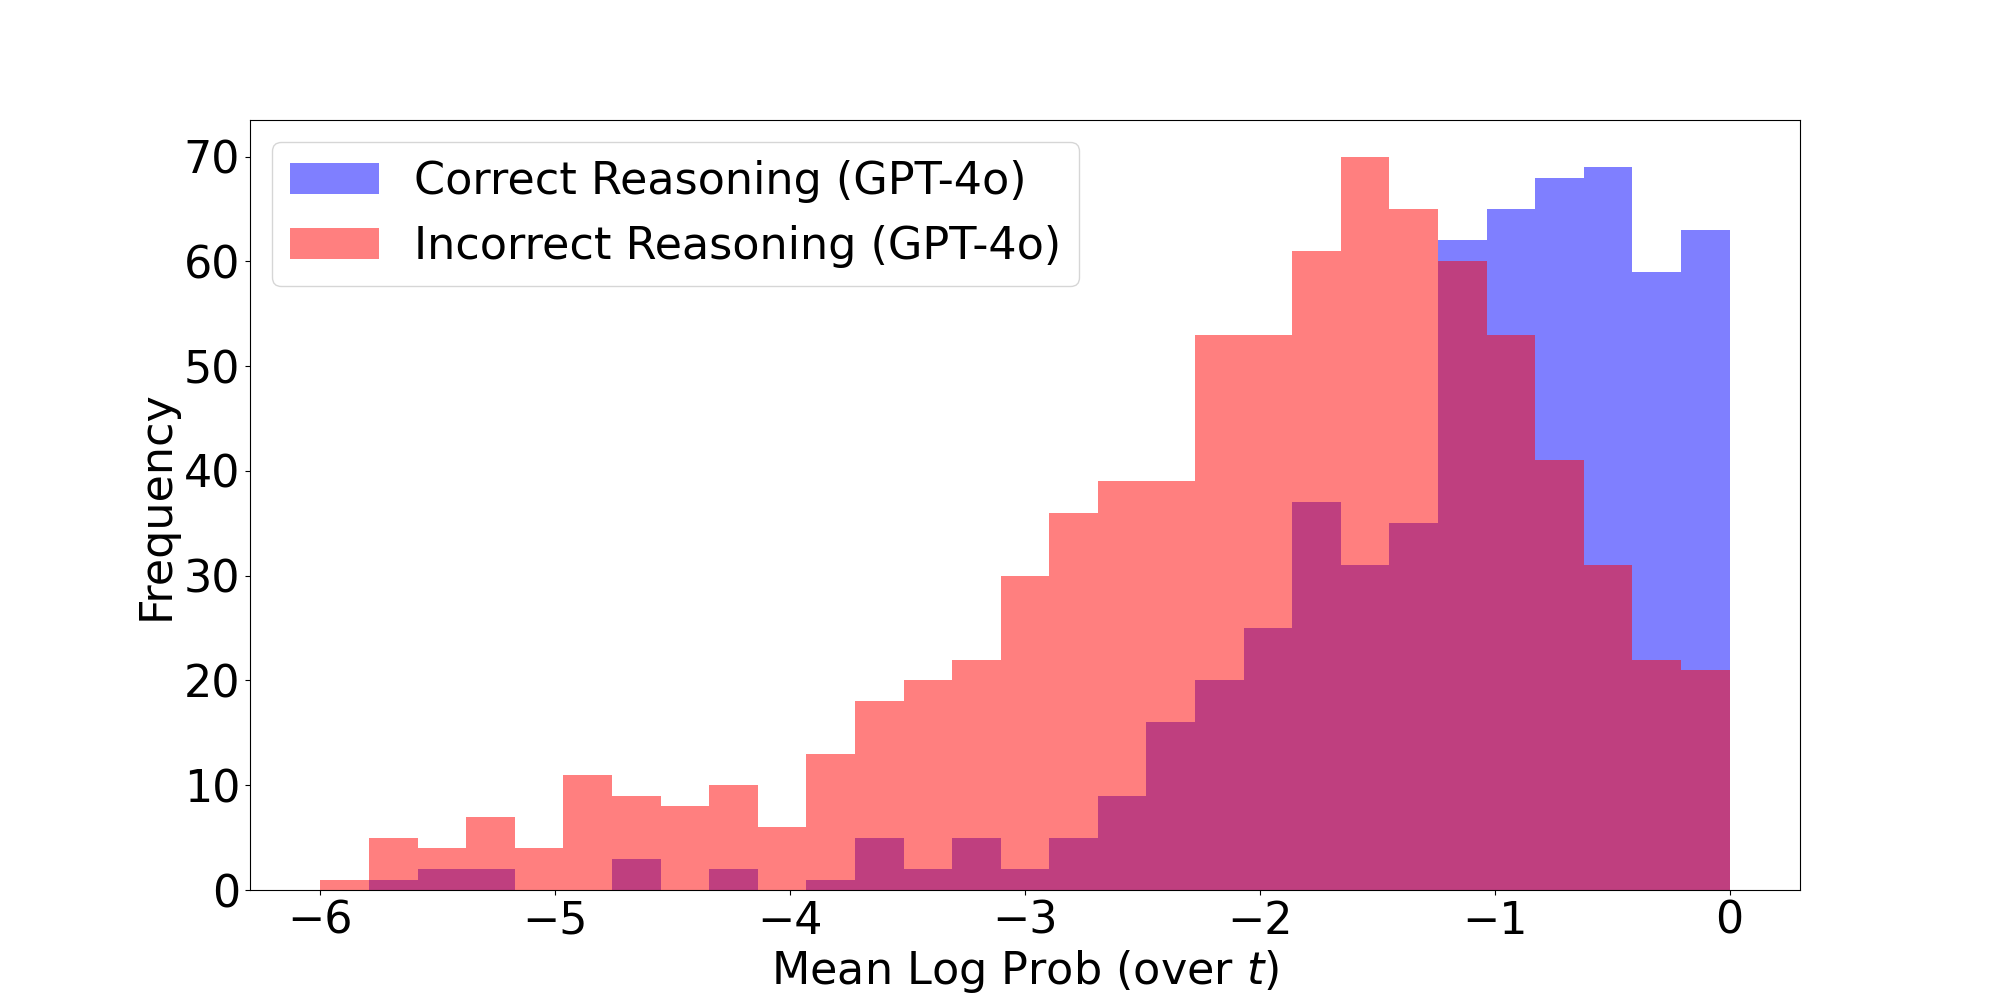
\includegraphics[width=0.9\linewidth]{plots/posterior_log_prob_distribution.png}
    \caption{\textbf{Distribution of answer block log probability scores for posterior samples.} To score the $1419$ posterior reasoning traces, we iteratively unmask each chain left-to-right, and compute the average answer block log probabilities across all timesteps. Posterior chains rated as correct by \textsc{GPT4}-o tend to have higher scores.}
    \label{fig:posterior_logprob_dist}
\end{figure}

\begin{figure}
    \centering
    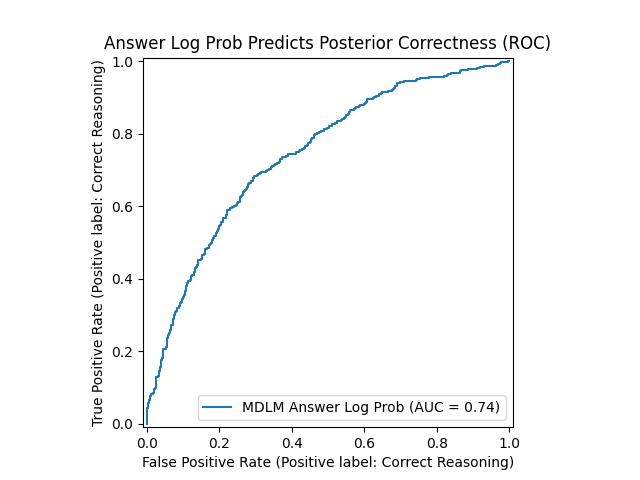
\includegraphics[width=0.6\linewidth]{plots/posterior_logprob_roc.png}
    \caption{\textbf{Answer block log probability scores predict posterior reasoning trace quality.} The \gls{mdlm} average answer block log probabilities can simply be thresholded to provide a classifier for predicting \textsc{gpt4}-o reasoning chain judgments. This classifier provides a potential method for filtering low-quality posterior samples (e.g. before fine-tuning).}
    \label{fig:posterior_logprob_roc}
\end{figure}


